\documentclass[a4paper, 12pt]{article} 
\usepackage{natbib}
\usepackage[utf8]{inputenc} %Pacote para acentuação
\usepackage[portuguese,brazilian]{babel}
\usepackage[lmargin=3cm,tmargin=3cm,rmargin=2cm,bmargin=2cm]{geometry} 
\usepackage[T1]{fontenc} %Ajusta o texto que vem de outras fonte
\usepackage{graphicx,xcolor,multirow,multicol}
\usepackage{amsmath,amsthm,amsfonts,amssymb,dsfont,mathtools}
\usepackage{blindtext}
\usepackage{indentfirst}
\usepackage{url}
\usepackage{quoting}
\usepackage{setspace}
\setlength{\parindent}{1.25cm}


\title{IF669 - Introdução a Programação}
\author{Marcelo Anderson Oliveira de Santana}
\date{Dezembro, 2021}

\begin{document}


\maketitle

\section{Introdução}
\subsection{Sobre a disciplina}
O projeto aborda sobre a disciplina “Introdução a Programação”, ministrada no curso de graduação de Ciência da Computação, da Universidade Federal de Pernambuco. Como forma de desenvolver o raciocínio lógico e introduzir os alunos à programação, a disciplina adota \textit{Python} como linguagem utilizada, sendo a mesma de tipagem dinâmica. Além do mais, 'IP' possui uma carga horária total de 120h, é obrigatória na grade curricular do discente e possui crédito 6. 

\subsection{Sobre a Metodologia de Ensino}
Sobre a metodologia de ensino, três professores ministram a disciplina, revezando entre si. O sistema de notas é divido em: $70\%$ são listas de treinamento e $30\%$ correspondem ao miniprojeto no final do semestre. 
Têm-se duas plataformas de estudos: o \textit{Dikastis}, sendo o ambiente onde são postadas as listas de treinamento que compõem a nota, e o \textit{Redu}, plataforma na qual tem o conteúdo semanal, em forma de vídeo e por cadernos de \textit{Jupyter Notebook}.

A forma de contato se dá principalmente pelos horários de aula síncronas, nas quais os monitores tiram dúvidas dos estudantes, e também pelo servidor do Discord, onde também existe meio de comunicação entre os discentes e os professores.

\section{Conteúdos}
A forma de realizar um algoritmo dentro das diferentes linguagens de programação é o que faz com que elas sejam diferentes entre si, ou seja, a sintaxe de uma linguagem para outra é diferente, mas o que se quer resolver, não. Por isso, durante todo o semestre da disciplina, são estudadas estruturas gerais, presentes em grande parte das linguagens. 

O que diferenciam essas linguagens é a maneira de escrever o código para execução de algum comando específico, sendo esse comando, em sua grande maioria, presente em outra linguagem, diferindo apenas na maneira de utilizá-lo.

Abaixo, seguem os comandos abordados durante o semestre, juntamente com uma breve explicação do que os mesmos podem realizar.

\subsection{Comandos Condicionais}
Os comandos condicionais são utilizados quando queremos analisar uma certa expressão e, a partir desse resultado, executar certo bloco de código que está identado nessa condição.

Em \textit{Python}, para estruturas condicionais, têm-se o \textit{if, elif} e \textit{else}. O \textit{if}, como a própria tradução do Inglês já diz, executa aquele código \textbf{se} tal proposição for verdadeira. 

Em alguns casos, temos várias condições dependentes, e são nesses casos que usamos o \textit{elif}: quando uma primeira proposição não é verdadeira, a elaboração de outra expressão dependente do resultado da primeira é feita por esse comando. 

Por último, caso nenhuma das condições tenham sido verdadeiras, temos a estrutura \textit{else} (no Português, “senão”), que executa um bloco de código caso nenhuma das outras condições não tenham sido realizadas. 

\begin{figure}[ht]
    \centering
    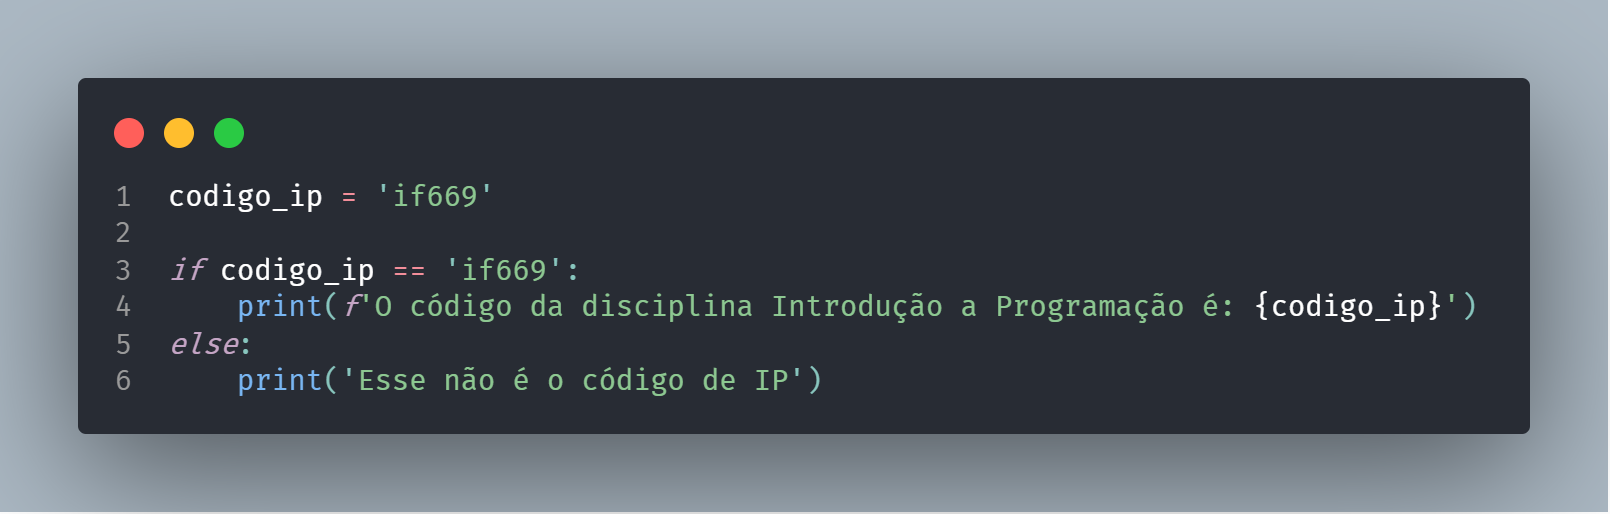
\includegraphics[width = 12cm]{imagens/if.png}
    \caption{Exemplo de código com estruturas condicionais \cite{codes}}
    \label{If's}
\end{figure}
O resultado desse código será a impressão da frase "O código da disciplina Introdução a Programação é: if669", pois a primeira condição foi satisfeita. 

O comando \textit{print} é utilizado para dar saída, ou seja, fornecer um \textit{output} para o usuário.

\subsection{Laços de Repetição}
Existem algumas instruções dentro do nosso algoritmo  que precisam ser executadas várias vezes seguidas no decorrer do código. Quando isso acontece, essa situação é chamada de \textit{loop}. Para tal, no \textit{Python}¸ têm-se dois comandos de repetição: o \textit{for} e o \textit{while}. O primeiro é geralmente usado quando se quer percorrer alguma coleção de dados, já o \textit{while} é utilizado enquanto uma condição é verdadeira. 

De maneira mais geral, é sempre explicado que o \textit{for} é mais recomendável quando queremos iterar sobre uma sequência de dados. \cite{loops} 


\begin{figure}[ht]
    \centering
    \begin{minipage}{0.5\textwidth}
        \centering
        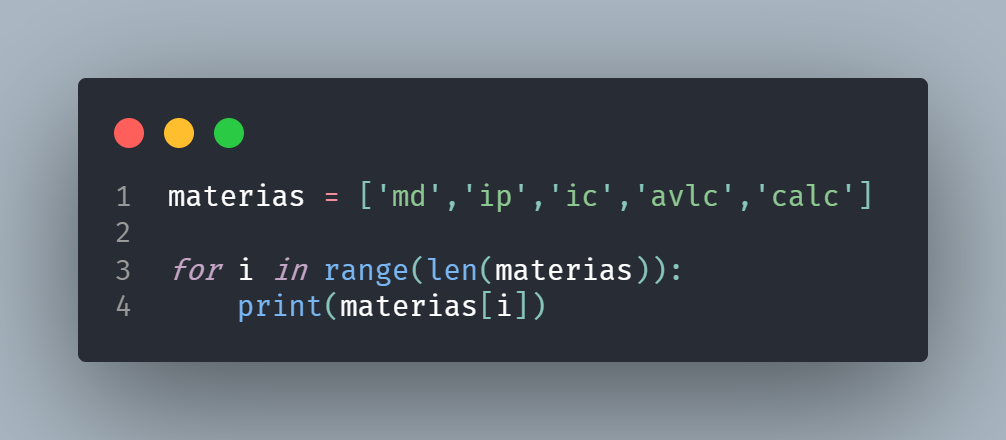
\includegraphics[width=0.95\textwidth]{imagens/loop_for.png} 
        \caption{\textit{Loop} com \textit{for}}
        \label{loop_for}
    \end{minipage}\hfill
    \begin{minipage}{0.5\textwidth}
        \centering
        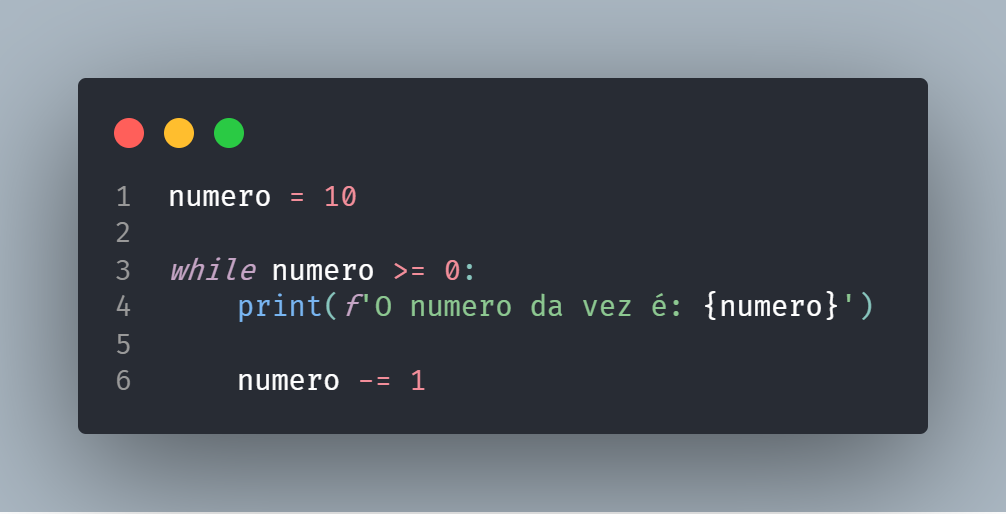
\includegraphics[width=0.8\textwidth]{imagens/loop_while.png}
        \caption{\textit{Loop} com \textit{while}}
        \label{loop_while}
    \end{minipage}
\end{figure}
Como pode ser observado nas imagens, a \ref{loop_for} imprime todos os valores que estão dentro da lista "materias", incremetando o valor de 'i' a cada execução.

Já a \ref{loop_while} imprime o numero da vez enquanto o mesmo é maior ou igual a zero. Quando o numero for igual a $-1$, por exemplo, o \textit{loop} não irá rodar mais.

O comando \textit{len}, na figura \ref{loop_for} serve para mensurar o comprimento da lista, ou seja, para o valor i durante toda a extensão da lista materias, imprima o índice atual da lista.

\subsection{Listas}
\label{Listas}
Como visto no \textit{loop "for"} do tópico anterior, listas são sequências de objetos, separados por vírgula e com começo e fim sinalizados através de colchetes. São utilizadas para armazenar diferentes valores, inclusive podem receber tipos de elementos variáveis.

\begin{figure}[ht]
    \centering
    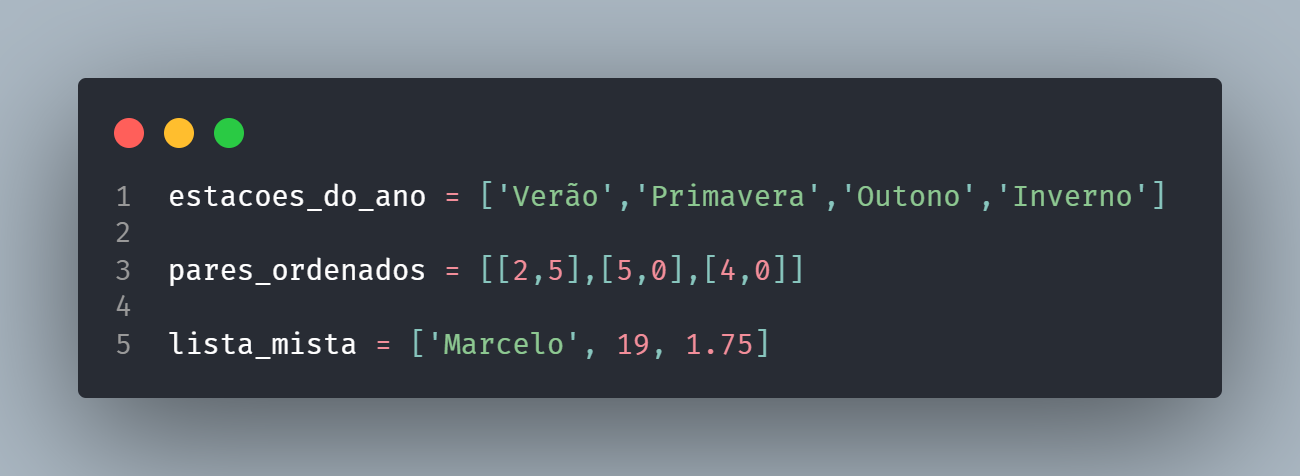
\includegraphics[width = 12cm]{imagens/listas.png}
    \caption{Listas em \textit{Python}}
    \label{listas}
\end{figure}

Na figura \ref{listas}, pode-se observar três tipos de Listas:
\begin{enumerate}
    \item A primeira lista só recebe valores em \textit{strings} e armazena as estações do ano;
    \item A lista $2$ armazena coordenadas de um sistema X,Y. Pode-se notar, nesse exemplo, que existem listas dentro da lista maior;
    \item No último exemplo, são armazenados diferentes tipos de variáveis na lista.
\end{enumerate}

É importante dizer que listas são estruturas mutáveis, ou seja, podem ser ascrescentadas de valores novos (isso é feito através do comando '\textit{append}'), como também podem ser retirados valores dessa sequência (por meio do comando '\textit{remove}').

\subsection{Funções}
\label{Funções}
Funções podem ser definidas como blocos de código que executam certa tarefa toda vez que são invocados no desenvolvimento do código. Isso significa que, ao criar um programa e realizar uma sequência de ações, esse mesmo processo pode ser realizado posteriormente no código ao defini-lo dentro de uma funçao. Basta, para executar aquela instrução novamente, invocar a função.

A sintaxe de uma função é feita por três partes: nome, parâmetros e corpo. O nome é importante para identificar a função, os parâmetros são os elementos necessários que aquela função precisa para ser executada, e o corpo é exatamente o que vai ser feito por essa estrutura. 
\begin{figure}[!h]
    \centering
    \includegraphics[width = 10cm]{imagens/funçao.png}
    \caption{Exemplo de Função}
    \label{função}
\end{figure}

\pagebreak
Na figura \ref{função}, podemos notar a definição de uma função com nome 'imprimir', que tem como parâmetros 'nome', 'idade' e 'trabalho'. Logo após, temos o corpo da função e, na linha 10, temos a chamada da função para executar suas instruções. Sempre que for necessário chamar essa função, basta apenas digitar seu nome e seus parâmetros.

\subsection{Recursão}

De acordo com o "Pense\textit{Python}",

\begin{quoting}[rightmargin=0cm,leftmargin=4cm]

\begin{singlespace}
    {\footnotesize 
    Recursão é 'um método de resolução de problemas que envolve quebrar um problema em subproblemas menores e menores até chegar a um problema pequeno o suficiente para que ele possa ser resolvido trivialmente. Normalmente recursão envolve uma função que chama a si mesma. Embora possa não parecer muito, a recursão nos permite escrever soluções elegantes para problemas que, de outra forma, podem ser muito difíceis de programar.' \cite{recursao}
    }
\end{singlespace}

\end{quoting}

A recursão tem 2 fatores principais:
\begin{enumerate}
    \item Caso básico: quando a função vai parar
    \item Casos recursivos: execução da função e chamada dela novamente, mudando os valores.
\end{enumerate}

Como visto no tópico \ref{Funções}, uma função funciona como um método bastante importante para se criar nos códigos, podendo ser reutilizada durante todo o algoritmo. Por isso, criar uma recursão para essa função é muito mais intuitivo e enxuto em comparação com a criação de \textit{loops}.

\begin{figure}[ht]
    \centering
    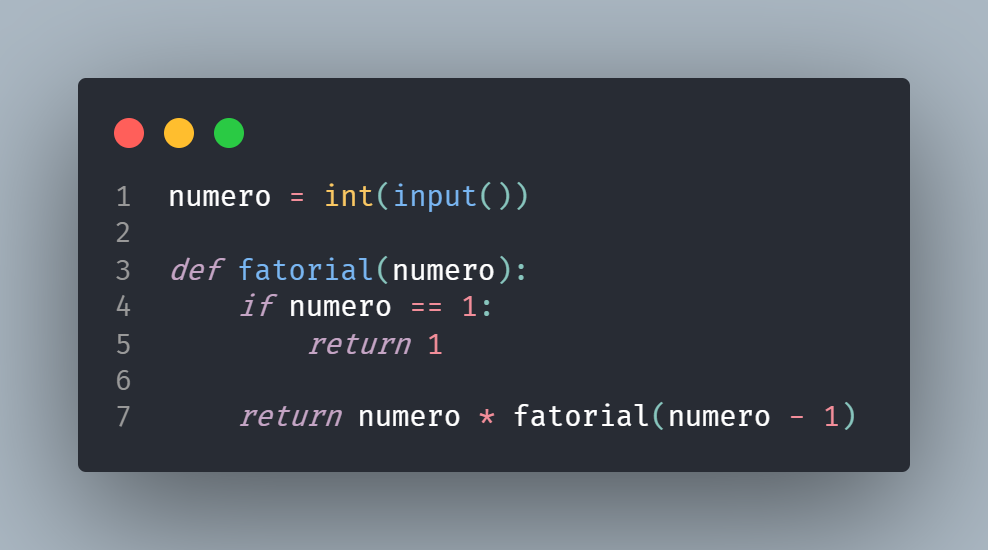
\includegraphics[width = 10cm]{imagens/recursao.png}
    \caption{Função recursiva em \textit{Python}}
    \label{recursao}
\end{figure}

\pagebreak
O caso da Figura \ref{recursao} mostra a elaboração de uma função recursiva para cálculo do fatorial de um número inteiro.

A abreviação 'int' na variável 'número' significa que esse valor será do tipo inteiro, e o comando '\textit{input}' pede para o usuário digitar algum número. Após isso, tem-se a função 'fatorial', que calculará, a partir do \textit{input}, o fatorial desse número,

\subsection{Tuplas}
Tuplas são estruturas de dados que também são capazes de armazenar dados, mas, diferentemente das Listas (abordadas no tópico \ref{Listas}, as tuplas são imutáveis, garantindo maior segurança no armazenamento de dados.

É possível, por exemplo, dizer que Getúlio Vargas não foi um dos presidentes do Brasil? Definitivamente não. Por isso, é mais viável armazenar esse tipo de informação dentro de uma estrutura que não é mutável e que garante que aqueles valores não serão modificados, e para isso temos a tupla.

\begin{figure}[ht]
    \centering
    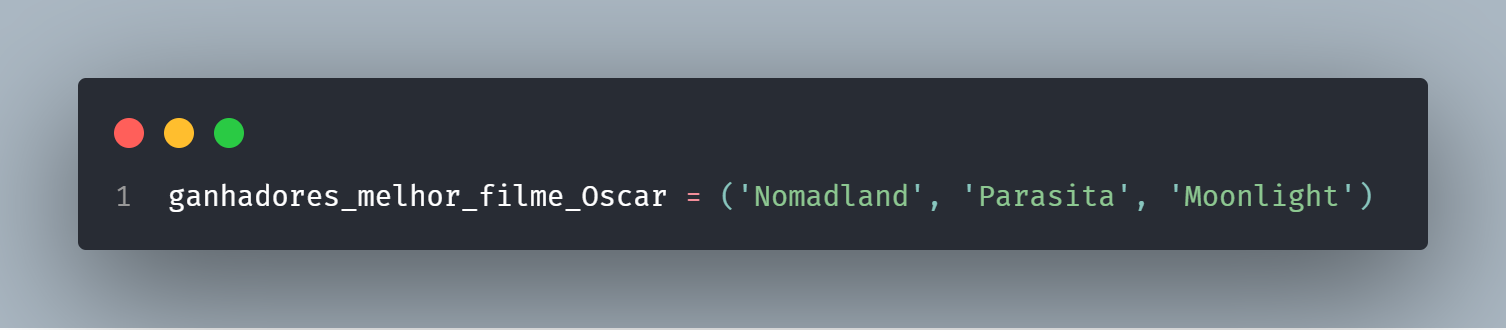
\includegraphics[width = 13cm]{imagens/tupla.png}
    \caption{Tupla em \textit{Python}}
    \label{tuplas}
\end{figure}
Na figura acima, é inegável que tais filmes foram ganhadores da categoria 'Melhor Filme' em algumas edições do Oscar.

\subsection{Dicionários}

Se é desejado para o programa armazenar chaves e valores correspondentes para elas, existem os dicionários. 

Essa estrutura de dados servem para armazenar uma chave e o(s) atributo(s) da mesma. Por exemplo, dentro do contexto da Figura \ref{tuplas}, caso fosse necessário salvar todos os ganhadores de todas as categorias do Oscar 2019? Como isso poderia ser feito?. 

O dicionário receberia, como chaves, todas as categorias, e os valores dessas chaves seriam os vencedores. A figura abaixo mostra, brevemente, como seria esse dicionário. 

\begin{figure}[ht]
    \centering
    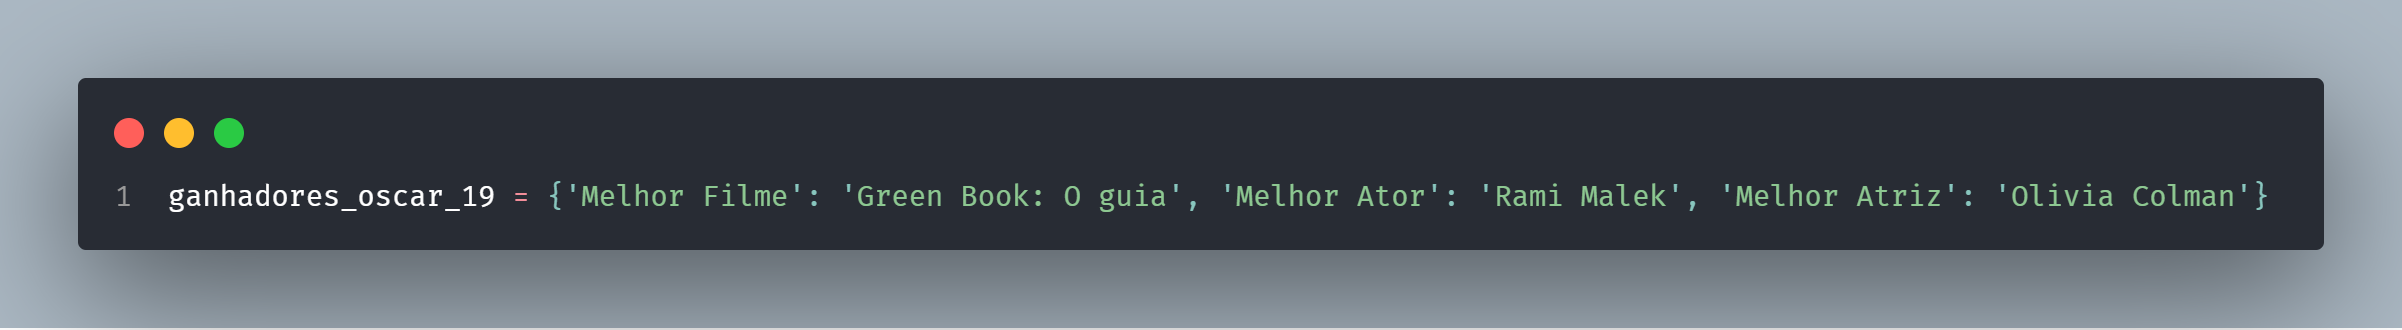
\includegraphics[width = 10cm]{imagens/dicionario.png}
    \caption{Exemplo de dicionário \cite{oscar}}
    \label{Dicionário}
\end{figure}

\section{Relação com outras disciplinas e Relevância}
'Introdução a Programação' é uma disciplina que desenvolve o discente para toda a trajetória acadêmica, haja visto que a lógica de resolução das listas de exercícios é exigida e ainda mais estimulada na cadeira 'Lógica para Computação', novos algoritmos e maior detalhamento sobre eles serão estudados em 'Algoritmos e Estrutura de Dados', assim como a maneira que a máquina lê o programa desenvolvido é visto na disciplina de 'Infraestrutura de Software'. 

Além do mais, a definição de que \textit{Python} é uma linguagem com tipagem dinâmica se relaciona com palestras ministradas para a disciplina de 'Introdução a Computação', a recursão, utilizada em funções recursivas, é abordada em 'Matemática Discreta para Computação' na elaboração de provas concretas para o campo da Matemática. 

A disciplina 'Interface Usuário-Máquina' aborda, de acordo com o próprio site da cadeira \cite{ifm}, sobre “o escopo de conhecer as necessidades de um público e idealizar uma solução para a necessidade encontrada, conversando com pessoas que conhecem e/ou vivenciam o tema, para que a solução desenvolvida seja pertinente.” Portanto, os conhecimentos vistos em IP terão aplicação direta no progresso dessa disciplina. 

O gerenciamento de dados também é abordado introdutoriamente em IP, tendo em vista que alguns comandos só são executados a partir da recepção de dados do(s) usuário(s), e a forma como esses dados são usados é explorada de maneira mais expansiva na disciplina \textit{IF685}, 'Gerenciamento de Dados e Informação'.

Portanto, a conexão entre 'Introdução a Programação' e outras disciplinas é vasta, auxiliando o corpo discente na caminhada da graduação e também em projetos paralelos, assim como no mercado de trabalho.


\newpage
\bibliographystyle{unsrt}
\bibliography{referencias}
\end{document}